\documentclass[conference]{IEEEtran}

\IEEEoverridecommandlockouts
\usepackage{cite}
\usepackage{kotex}
\usepackage{float}
\usepackage{amsmath,amssymb,amsfonts}
\usepackage[ruled, vlined]{algorithm2e}
\usepackage{graphicx}
\usepackage{textcomp}
\usepackage{xcolor}
\usepackage{listings}
\usepackage{caption}
\usepackage{subcaption}
\usepackage{multirow}
\usepackage{booktabs}
\usepackage{makecell}
\usepackage{hyperref}
\hypersetup{
    colorlinks=true,
    linkcolor=blue,
    filecolor=magenta,
    urlcolor=cyan,
}
\urlstyle{same}
\newcommand{\tool}{{\sc JUSTGen}\xspace}

\lstset{basicstyle=\ttfamily}
%\newcommand{\tool}{\textsf{\small JEST}}

\begin{document}

\title{JUSTGen: Effective Test Generation for Unspecified JNI Behaviors on JVMs}
%\title{$\textsf{JEST}$: $N\!+\!1$-version Differential Testing of\\
%  Both JavaScript Engines and Specification}

\author{\IEEEauthorblockN{Sungjae Hwang}
\IEEEauthorblockA{
  \textit{School of Computing} \\
\textit{KAIST}\\
Daejeon, South Korea \\
sjhwang87@kaist.ac.kr}

\and

\IEEEauthorblockN{Sungho Lee}
\IEEEauthorblockA{
  \textit{Department of Computer Science and Engineering} \\
\textit{Chungnam National University}\\
Daejeon, South Korea \\
eshaj@cnu.ac.kr}

\and

\IEEEauthorblockN{Jihoon Kim}
\IEEEauthorblockA{
  \textit{School of Computing} \\
\textit{KAIST}\\
Daejeon, South Korea \\
kjh618@kaist.ac.kr}

\and

\IEEEauthorblockN{Sukyoung Ryu}
\IEEEauthorblockA{
  \textit{School of Computing} \\
\textit{KAIST}\\
Daejeon, South Korea \\
sryu.cs@kaist.ac.kr}
}

\maketitle

\begin{abstract}
Java Native Interface (JNI) provides a way for Java applications to access native libraries,
but it is difficult to develop correct JNI programs.
By leveraging native code, the JNI enables Java developers to implement efficient applications 
and to reuse code written in other programming languages such as C and C++. 
Besides, the core Java libraries already use the JNI to provide system features like
a graphical user interface. As a result, many mainstream Java Virtual
Machines (JVMs) support the JNI. 
However, due to the complex interoperation semantics between different programming languages, 
implementing correct JNI programs is not trivial.
Moreover, because of the performance overhead, JVMs do not validate
erroneous JNI interoperations by default, but they validate them only when
the debug feature, the \emph{-Xcheck:jni} option, is enabled.
Therefore, the correctness of JNI programs highly relies on the checks
by the -Xcheck:jni option of JVMs.
Questions remain, however, on the quality of the checks provided by the feature.
Are there any properties that the -Xcheck:jni option fails to validate? 
If so, what potential issues can arise due to the lack of such validation? 
To the best of our knowledge, no research has explored these questions in-depth.
  
In this paper, we empirically study the validation quality and impacts
of the -Xcheck:jni option on mainstream JVMs using unspecified corner cases in the JNI specification. 
Such unspecified cases may lead to unexpected run-time behaviors
because their semantics is not defined in the specification. 
For a systematic study, we propose \tool, a semi-automated approach
to identify unspecified cases from a specification and generate test programs. 
\tool receives the JNI specification written in our domain specific language (DSL),
and automatically discovers unspecified cases using an SMT solver. 
It then generates test programs that trigger the behaviors of unspecified cases. 
Using the generated tests, we empirically study the validation ability
of the -Xcheck:jni option.
Our experimental result shows that the JNI debug feature does not validate thousands 
of unspecified cases on JVMs, and they can cause critical run-time errors
such as violation of the Java type system and memory corruption. 
We reported 792 unspecified cases that are not validated by JVMs to
their corresponding JVM vendors.  Among them, 563 cases have been
fixed and the remaining cases will be fixed in near future. 
Based on our empirical study, we believe that the JNI specification should specify 
the semantics of the missing cases clearly and the debug feature should be supported
completely.
\end{abstract}

\begin{IEEEkeywords}
Java Native Interface, Java Virtual Machine, Testing, Empirical Study, Debugging
\end{IEEEkeywords}

\section{Artifact Description}

\begin{figure*}
  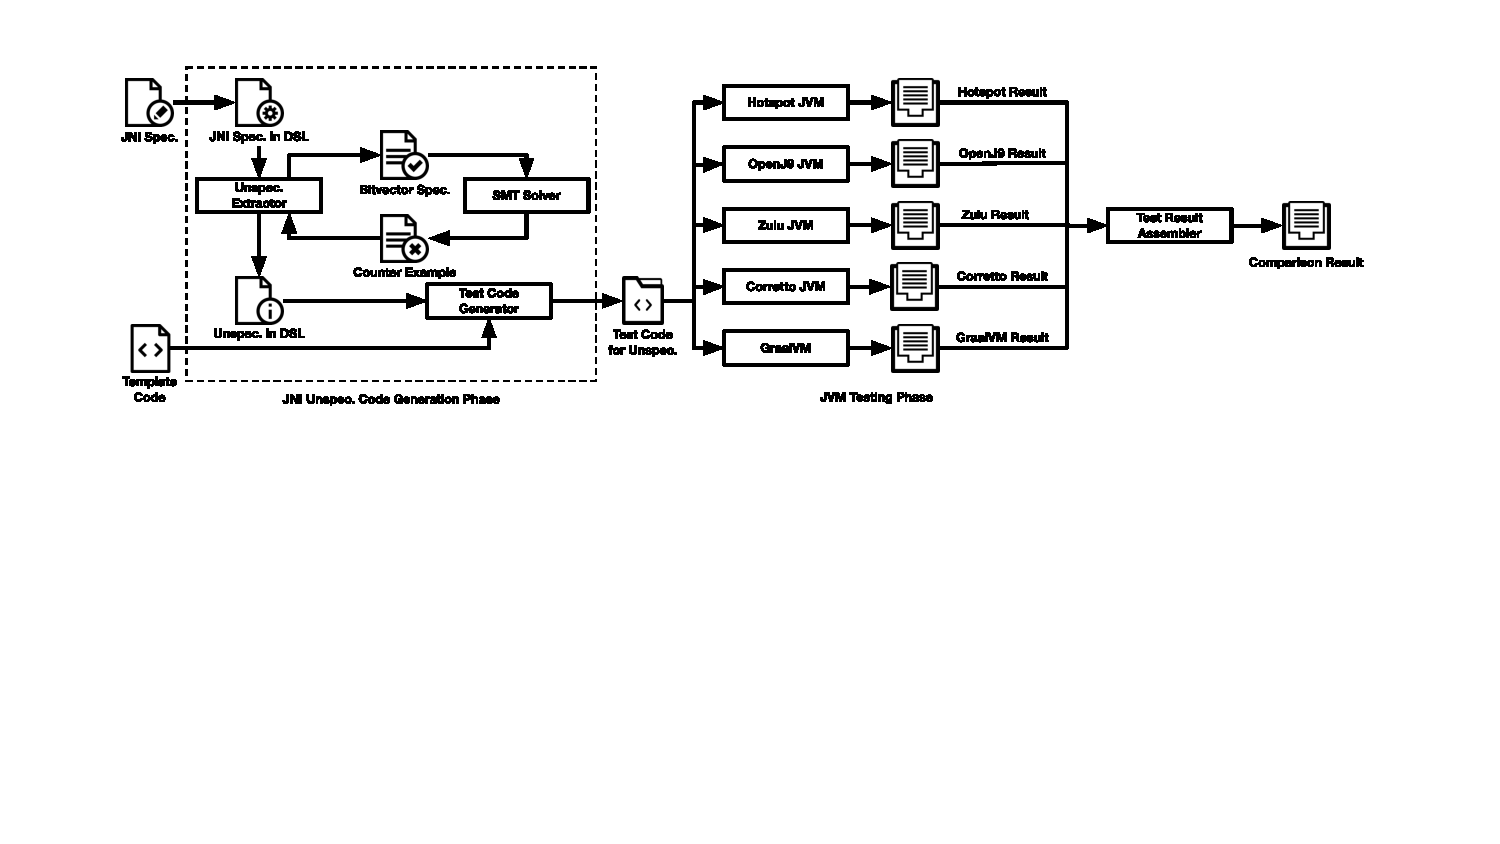
\includegraphics[width=0.98\textwidth]{dsl_overview5.pdf}
  \caption{Overall structure of JUSTGen}
  \label{fig:overall}
\end{figure*}

JUSTGen is a framework that consists of two parts. The first part identifies 
unspecified cases from the JNI specification expressed in our DSL (Domain Specific Language). 
The second part generates test programs triggering the behaviors of the identified unspecified cases. 
As shown in Figure~\ref{fig:overview}, the artifact consists of following modules:

\begin{itemize}
  \item \textbf{Unspec. Extractor} finds unspecified cases from the JNI specification expressed in our DSL. 
  \item \textbf{Test Code Generator} generates test programs triggering identified unspecified cases
  
\end{itemize}

\section{Getting Started Guide}

The artifact is open-source can be obtained by cloning the following git
repository:
\begin{lstlisting}
$ git clone \ 
  https://github.com/sjmini/justgen.git 
\end{lstlisting}
To build and execute the artifact, you should follow the instrucitons in the
\texttt{INSTALL} file in the artifact. 
Since the tool is using a SMT solver when finding unspecified cases, Z3 is required.
Morevore, JUSTGen uses the Dune build system. 
JUSTGen can be easily built by just issuing \textit{make} command.
The required packages to build and run JUSTGen are summarized in \texttt{INSTALL} file.

\section{Artifact Structure}

The artifact consists of following files:

\begin{lstlisting}
1.test/rule: JNI spec expressed in our DSL 
2.test_case: Location of Test programs
3.slang.exe: Executable file of JUSTGen
4.src: Source files of JUSTGen
5.test/bitvector: predefined bitvectors
6.test/refine_meaning: refinements info 
7.test/code/*: Template codes
8.unspec_dsl: unspecified cases in DSL 
9.gen_result: identified unspecified cases
\end{lstlisting}

\section{Basic Commands}

You can run the artifact with the following command to find unspecified cases:
\begin{lstlisting}
$ ./slang.exe find_unspec |tee unspec_dsl
\end{lstlisting}

You can generate test programs triggering the behaviors of identified unspecified cases with the following command:
\begin{lstlisting}
$ ./slang.exe gen_program |tee gen_result
\end{lstlisting}

Note that the \textit{unspec\_dsl} file must be generated by running \textit{find\_unspec} option before executing the JUSTGen with \textit{gen\_program} option.
The test programs will be placed in \textit{test\_case} folder.

\section{Tool Output}
Currently, the JNI specification expressed in our DSL defines 37 types and 105 refinement types. 
Based on this JNI specification, the JUSTGen finds 34,990 unspecified cases.
The unspecified cases can be found in \textit{gen\_result} file.

By running the generated test programs, you can test JNI behaviors of JVM. 
If you change the content of test/rule file according to the targeted specification, 
the JUSTGen will find the new unspecified cases.

\section{Bug Report}
Using 34,990 test programs generated by JUSTGen, 
we empirically evaluated the \textit{-Xcheck:jni} option on five mainstream JVMs.
We found following bugs and limitations from JVMs.

\begin{lstlisting}
github.com/eclipse/openj9/issues/10183
github.com/eclipse/openj9/issues/9452
github.com/eclipse/openj9/issues/10191
github.com/eclipse/openj9/issues/10210
github.com/eclipse/openj9/issues/10231
github.com/eclipse/openj9/issues/10272
github.com/eclipse/openj9/issues/10286
github.com/eclipse/openj9/issues/10310
github.com/eclipse/openj9/issues/10318
github.com/eclipse/openj9/issues/10473
github.com/eclipse/openj9/issues/10476
github.com/eclipse/openj9/issues/10477
github.com/eclipse/openj9/issues/10479
github.com/eclipse/openj9/issues/10480
github.com/oracle/graal/issues/2815
github.com/corretto/corretto-11/issues/128
github.com/eclipse/openj9/issues/10481
github.com/eclipse/openj9/issues/10484
\end{lstlisting}

Our study shows that many of the unspecified cases are not validated by JVMs, 
and they can cause critical run-time errors such as run-time type errors and memory corruption. 
In addition, we found a bug of the \textit{-Xcheck:jni} option, 
which leads to deadlock between multiple threads.

\end{document}
